\documentclass{article}
\usepackage{iclr2026_conference,times}

\usepackage{amsmath,amssymb,amsthm}
\usepackage{graphicx}
\usepackage{booktabs}
\usepackage{multirow}
\usepackage{xcolor}
\usepackage{hyperref}
\usepackage{url}

\newtheorem{proposition}{Proposition}
\newcommand{\dr}{d_r}
\newcommand{\dc}{d_c}
\newcommand{\ceff}{c_{\mathrm{eff}}}
\newcommand{\R}{\mathbb{R}}
\newcommand{\ip}[2]{\langle #1, #2\rangle}

\title{The Compounding Bottleneck: A Unified Capacity Account of\\ Retrieve-then-Compress Retrieval-Augmented Generation}

\author{Anonymous authors\\Paper under double-blind review}

%\iclrfinalcopy % <-- UNCOMMENT for the camera-ready (de-anonymized) version.
\newcommand{\fix}{\marginpar{FIX}}
\newcommand{\new}{\marginpar{NEW}}

\begin{document}
\maketitle

\begin{abstract}
Efficient retrieval-augmented generation (RAG) funds two fixed-dimensional vector bottlenecks
out of one budget: the dense-retrieval embedding of dimension $\dr$, and the soft-context
compression code of size $m\!\cdot\!\dc$. Prior work bounds the retrieval stage or studies
compression overflow, but never the composition. We give a unified capacity account that treats
both stages as thresholded-separation problems of the same geometric form, and we make four
observations, each validated from controlled free-vector geometry up to production encoders.
First, the two stages carry sharp capacity walls whose critical dimension grows with content;
the retrieval wall replicates across two embedder families, two datasets, and optimal (PCA)
truncation, and on the adversarial LIMIT benchmark three real embedders collapse to
$2.8\!-\!8.2\%$ recall@100. Second, composing the stages \emph{compounds}: the best split of a
shared budget underperforms either stage given the full budget, and the sign of the deviation
from the product law is governed by the correlation $\rho$ between which items are hard to
retrieve and which are hard to compress. Third, we measure $\rho$ on a real pipeline and find
$\rho\!\approx\!0$, so real RAG sits in the multiplicative regime and a simple product-law
allocation is near-exact; the allocation is interior, which we confirm both on a synthetic corpus and
on a real multi-hop QA benchmark with a frozen reader scored by EM/F1 (a single-peaked allocation
curve and a $0.048$ F1 compounding gap at a tight budget, over three seeds), and deployed
big-embedder/tiny-compressor configurations sit far off the frontier. Fourth, a multi-view
``facet-lens'' escapes the wall in
the free-vector worst case, but we show honestly that the escape does not transfer to strong real
encoders, which redirects the practical lever back to allocation. All claims are reproducible from
committed configurations.
\end{abstract}

\section{Introduction}

Retrieval-augmented generation has settled into a common efficient template: a query is embedded
and matched against a corpus by a dense retriever \citep{karpukhin2020dpr,lewis2020rag}, the
top passages are compressed into a handful of soft tokens so the generator pays little attention
cost \citep{mu2023gist,ge2023icae,cheng2024xrag}, and a frozen decoder answers from those tokens.
Both stages are, at heart, a fixed-dimensional vector bottleneck: retrieval squeezes relevance
through an embedding of dimension $\dr$, and compression squeezes a passage through a code of size
$m\!\cdot\!\dc$. The two bottlenecks are usually studied apart. On the retrieval side, a line of
work now argues that a $\dr$-dimensional single-vector index cannot realize arbitrary
top-$k$ relevance patterns, and \citet{weller2025limit} make this precise by tying feasibility to
the sign-rank of the relevance matrix and by building the LIMIT stress test on which frontier
models fail. On the compression side, \citet{belikova2026overflow} observe empirically that soft
tokens ``overflow'' past a finite capacity, and \citet{selecom2026} argue on information-theoretic
grounds that full compression is neither feasible nor necessary, yet decline to give a capacity
bound or to connect compression back to the embedding-dimension wall.

What has been missing is the composition. Efficient RAG runs the compressor on the \emph{output}
of the retriever, so the two capacity-limited stages act in series, and the natural question is
whether their errors simply add, or whether stacking two bottlenecks does something worse. We find
that they \emph{compound}: there are inputs on which retrieval alone succeeds and on which
compressing the gold passage alone succeeds, and yet the composed pipeline fails, and the size of
this effect is predictable from the geometry of the two representations rather than from either
stage's standalone metric. This breaks the field's implicit assumption that retrieval error and
compression error are independent and additive, and it has a direct practical consequence, since a
budget spent overwhelmingly on a large embedding while the compressor is starved sits far from the
optimal allocation.

We organize the paper around four contributions, illustrated in Figure~\ref{fig:concept}. (C1) We
cast both stages as thresholded-separation problems of the same geometric form and show each has a
sharp capacity wall whose critical dimension grows with content; the retrieval wall is not an
artifact of one embedder, one dataset, or one truncation scheme, and it appears in full force on
Weller's own adversarial data. (C2) We show that composing two sub-full stages compounds, we
characterize the deviation from the product law through a hardness-correlation $\rho$, and---going
beyond the prior framing that left $\rho$ hypothetical---we \emph{measure} it on a real pipeline
and find it near zero, which places real RAG squarely in the multiplicative regime. (C3) Under a
fixed shared budget we derive and validate the optimal split, on synthetic corpora and end-to-end
on real encoders, and show that deployed configurations are off the frontier. (C4) We test the
obvious escape---a multi-view facet-lens that gives each semantic facet its own low-rank
subspace---and report the honest result that it escapes the wall in the free-vector worst case but
\emph{not} on strong real encoders, which we explain and which sharpens rather than weakens the
account. Every headline number is validated twice, from a free-vector best case that upper-bounds
any encoder to production embedders, and the negatives are reported alongside the positives because
they are what map the boundary of the effect.

\begin{figure}[t]
\centering
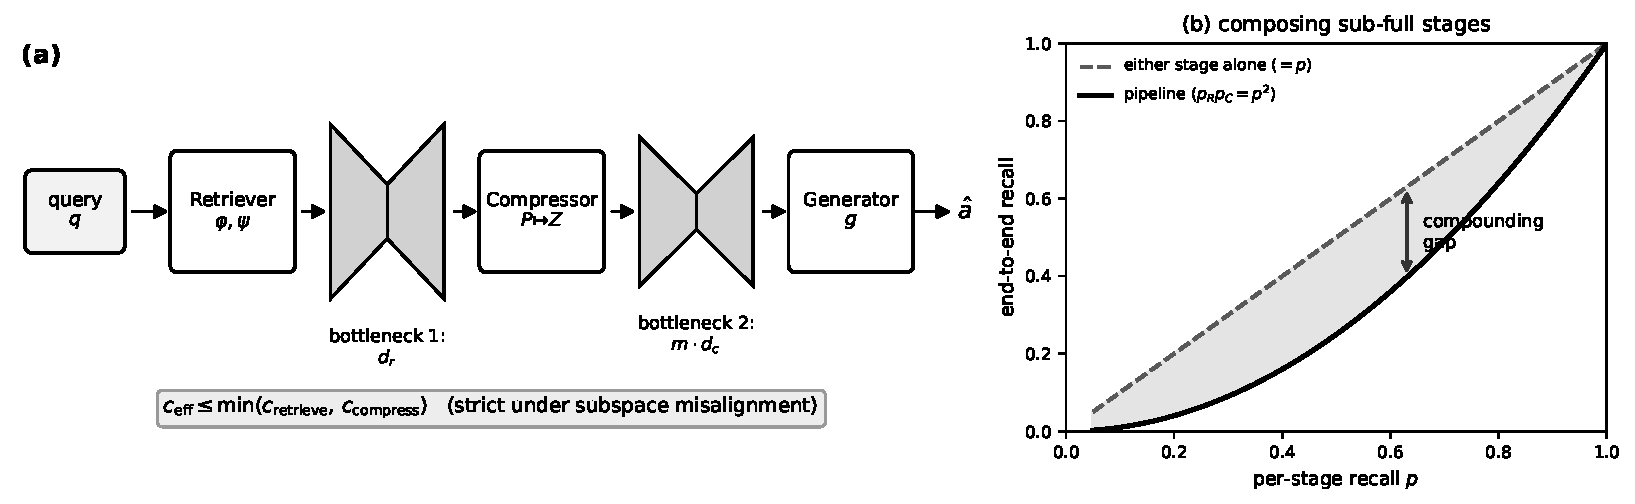
\includegraphics[width=\linewidth]{figures/fig1_concept.pdf}
\caption{\textbf{The compounding bottleneck.} (a) Efficient RAG passes a query through two
fixed-dimensional vector bottlenecks in series---the retrieval embedding ($\dr$) and the soft
compression code ($m\!\cdot\!\dc$)---so the realizable set is the intersection of two
subspace-constrained families and $\ceff\le\min(c_{\mathrm{retrieve}},c_{\mathrm{compress}})$,
strict under generic misalignment. (b) Composing two stages that each achieve recall $p<1$ yields
$p_R p_C$ under independence, which lies below either stage alone; the shaded region is the
compounding gap.}
\label{fig:concept}
\end{figure}

\section{Related work}

\paragraph{Limits of dense retrieval.} That a fixed embedding dimension caps what a single-vector
retriever can express is the premise we build on. \citet{weller2025limit} connect the number of
realizable top-$k$ document subsets to embedding dimension through sign-rank
\citep{razborov2010signrank,forster2002linear} and release LIMIT, where even strong models score
low; scaling studies of embedding dimension in IR and analyses of granularity failures point the
same way. Matryoshka representation learning \citep{kusupati2022matryoshka} makes the leading
coordinates of an embedding independently useful, which is exactly what lets us trace the wall by
truncation on a real encoder. Multi-vector late interaction \citep{khattab2020colbert,
santhanam2022colbertv2} is the known partial escape from the single-vector bound, and we position
our facet-lens against it. Standard dense retrievers and embedders we use or reference include
\citet{reimers2019sbert,karpukhin2020dpr,izacard2022contriever,wang2022e5,li2023gte,xiao2023bge,
merrick2024arctic,ni2022gtr}, benchmarked in the style of \citet{thakur2021beir,muennighoff2023mteb}.

\paragraph{Context and soft-prompt compression.} Soft-compression methods replace a passage with a
few learned vectors read by a frozen decoder: Gist tokens \citep{mu2023gist}, in-context
autoencoding \citep{ge2023icae}, context-adapted models \citep{chevalier2023autocompressor}, and
one-token extreme compression \citep{cheng2024xrag}, alongside hard-prompt pruning
\citep{jiang2023llmlingua,jiang2023longllmlingua,pan2024llmlingua2,li2023selective} and abstractive
compression \citep{xu2024recomp,li2024500x}. Closest to us, \citet{belikova2026overflow} detect an
``overflow'' regime where compressed tokens can no longer answer a query, and \citet{selecom2026}
argue that query-conditioned selection beats full compression; both stop short of a capacity law
and of any link to the retrieval wall. We supply that link and, crucially, the cross-stage
composition.

\paragraph{RAG systems.} The broader pipeline we abstract is instantiated by
\citet{lewis2020rag,guu2020realm,borgeaud2022retro,izacard2023atlas,izacard2021fid,ram2023ralm,
shi2024replug,asai2024selfrag}. Our contribution is orthogonal: not a better pipeline, but a
capacity account of why stacking two fixed-dimensional codes loses information that either stage
alone would keep, and what to do about it.

\section{Setup and the capacity primitive}
\label{sec:setup}

\paragraph{Notation.} A corpus is $D=\{d_1,\dots,d_N\}$ with queries $q$ and a ground-truth
relevance matrix $A\in\{0,1\}^{|Q|\times N}$, where row $i$ marks the documents relevant to query
$i$. The retrieval stage uses a document encoder $\varphi:d\mapsto x\in\R^{\dr}$ and a query
encoder $\psi:q\mapsto y\in\R^{\dr}$, scores by $s(q,d)=\ip{y}{x}$, and returns the top $k$.
Realizing $A$ by thresholding $Y X^\top$ is governed by the sign-rank of $2A-1$
\citep{weller2025limit}, which is the retrieval wall. The compression stage maps a passage $P$ to
$Z\in\R^{m\times \dc}$ ($m$ soft tokens of width $\dc$) that a frozen reader answers from; we cast
``can the reader recover the queried fact from $Z$ among distractors'' as a second
thresholded-separation problem with its own capacity $c_{\mathrm{compress}}$. Because the
compressor acts on the retriever's output, the two capacities compose by set intersection, which we
state as follows and validate empirically throughout the paper.

\begin{proposition}[Compositional capacity]
\label{prop:compose}
Let $\mathcal{R}_r$ be the family of relevance/answer patterns realizable by the retrieval stage at
capacity $c_{\mathrm{retrieve}}$, and $\mathcal{R}_c$ the family realizable by the compression stage
at $c_{\mathrm{compress}}$. A pattern is realized end-to-end only if the retriever surfaces the gold
set \emph{and} the compressor preserves the answer from it, so the pipeline's realizable family is
$\mathcal{R}_r\cap\mathcal{R}_c$ and its effective capacity satisfies
$\ceff=|\mathcal{R}_r\cap\mathcal{R}_c|\le\min(c_{\mathrm{retrieve}},c_{\mathrm{compress}})$.
Equality holds iff one family contains the other; generically it does not---the retriever's
\emph{discriminative} subspace and the compressor's \emph{reconstructive} subspace are misaligned---
so the inequality is strict, and the shortfall is the failure-transfer set we measure in
Section~\ref{sec:compound}.
\end{proposition}

\noindent The proof is immediate (a pattern in neither stage's realizable family cannot be realized
by their composition); the content is empirical, namely \emph{how far} below the minimum the
composition falls, which is exactly the compounding gap C2 quantifies.

\paragraph{The free-embedding capacity measure.} To measure capacity without confounding it with a
particular encoder's quality, we directly optimize unconstrained document and query vectors of a
given dimension to realize a target pattern, using a pairwise margin objective, and report the
fraction of queries for which every relevant document outranks every non-relevant one
(``realizability''). This is the best case for \emph{any} encoder of that dimension, so it
upper-bounds real models and isolates the geometric limit; where we later want a smoother signal we
report recall@$k$ instead. The same primitive drives the retrieval probe (optimize $\R^{\dr}$
vectors against a relevance pattern) and the compression probe (a slot-memory read head over $m$
codes of width $\dc$), which is what lets us compare the two walls on the same axis. All runs are
seeded and multi-seed for headline claims, and we report compute alongside accuracy; experiments
ran on single commodity GPUs (Kaggle T4/P100).

\section{Two walls of the same geometry (C1)}
\label{sec:walls}

\paragraph{The retrieval wall.} On the adversarial ``all-pairs'' pattern, where every document
pair is some query's gold set ($k=2$), free-embedding realizability shows a sharp phase transition
in $\dr$: for a corpus of $n_d=40$ it jumps from $0.38$ to $1.0$ between $\dr=4$ and $\dr=8$ across
three seeds with near-zero variance, and the critical dimension $\dr^\star$ moves outward as the
corpus grows. The growth is real but slow: on a five-seed, two-pattern sweep (all-pairs and random
$3$-subsets) $\dr^\star$ moves only from $8$ to $11$ as $n_d$ goes from $40$ to $400$, consistent
with a sub-logarithmic law (a power fit gives exponent $b\!\approx\!0.16\!-\!0.18$), and we note
honestly that a tidy ``$\dr^\star\!\propto\! d/n_d$'' sub-critical collapse we initially conjectured
does \emph{not} hold ($R^2=0.18$); what survives, and is all the allocation law needs, is that a
modest critical dimension exists and grows with content.

The wall is not a free-vector artifact. Truncating a Matryoshka encoder
\citep{kusupati2022matryoshka} and re-normalizing traces the same ramp-then-saturate curve on real
data: \texttt{mxbai-embed-large} on SciFact climbs recall@10 from $0.09$ to $0.87$ and is
statistically flat beyond $\dr\!=\!512$, so the top half of a $1024$-dimensional production
embedding is wasted budget. Table~\ref{tab:generality} shows this replicates across settings that
rule out the obvious objections: a \emph{second} embedder family (\texttt{arctic-embed-m}, $768$d)
reaches $97\%$ of full recall by $\dr\!=\!256$; a \emph{second} dataset (FiQA, a domain shift)
reaches $92\%$ by $\dr\!=\!256$; and under \emph{PCA} truncation---the optimal $\dr$-dimensional
linear subspace, not a Matryoshka ordering---\texttt{bge-large} saturates hard at $\dr\!=\!256$
($98.5\%$ of full, the top $768$ dimensions adding $0.013$), which is the cleanest wall of the set
and the one that kills the ``your wall is just Matryoshka'' reading.

Most tellingly, the wall appears on the field's own adversarial benchmark. On the full LIMIT set
\citep{weller2025limit} ($50$k documents, two gold per query) three real embedders collapse to
recall@100 of $0.028$, $0.082$, and $0.045$ (Table~\ref{tab:limit}); on the $46$-document LIMIT-small,
recall@10 is only $0.44\!-\!0.62$, i.e.\ returning ten of just forty-six documents still misses
half the gold. That three different embedder families fail together, and consistently, is what
makes this the wall of the single-vector \emph{paradigm} rather than any one model's quirk.

\begin{table}[t]
\caption{\textbf{The retrieval wall generalizes} across a second embedder, a second dataset, and
optimal (PCA) truncation. We report recall@10 at truncated dimension $\dr$ and the fraction of
full-dimension recall retained at $\dr\!=\!256$. In every case a modest $\dr$ captures the bulk and
the remaining dimensions add little.}
\label{tab:generality}
\centering\small
\begin{tabular}{@{}llccccccc@{}}
\toprule
Embedder / data (trunc.) & full $d$ & $\dr{=}16$ & $32$ & $64$ & $128$ & $256$ & full & @256/full\\
\midrule
mxbai / SciFact (Matryoshka)   & 1024 & 0.33 & 0.57 & --   & 0.79 & 0.83 & 0.87 & 95\%\\
arctic-m / SciFact (Matryoshka)& 768  & 0.18 & 0.39 & 0.59 & 0.75 & 0.82 & 0.85 & 97\%\\
mxbai / FiQA (Matryoshka)      & 1024 & 0.10 & 0.24 & 0.42 & 0.53 & 0.60 & 0.65 & 92\%\\
bge-large / SciFact (PCA)      & 1024 & 0.49 & 0.65 & 0.76 & 0.80 & 0.85 & 0.86 & 98.5\%\\
\bottomrule
\end{tabular}
\end{table}

\begin{table}[t]
\caption{\textbf{The wall on canonical adversarial data} (LIMIT, \citealp{weller2025limit}).
Full set: $50$k documents, $1000$ queries, two gold per query. All three real embedder families
collapse; the failure is a property of the single-vector paradigm, not a model quirk.}
\label{tab:limit}
\centering\small
\begin{tabular}{@{}lcccc|c@{}}
\toprule
& \multicolumn{4}{c}{LIMIT-full (50k docs)} & LIMIT-small (46)\\
Embedder & R@2 & R@10 & R@100 & R@1000 & R@10\\
\midrule
mxbai-embed-large & 0.004 & 0.010 & 0.028 & 0.103 & 0.441\\
arctic-embed-m    & 0.009 & 0.024 & 0.082 & 0.254 & 0.619\\
bge-base          & 0.007 & 0.015 & 0.045 & 0.163 & 0.492\\
\bottomrule
\end{tabular}
\end{table}

\paragraph{The compression wall.} The compression stage carries a wall of the same form. On
controlled passages of $n_f$ facts read from $m$ soft codes, slot-memory realizability transitions
at a critical code size $D_c^\star=m\!\cdot\!\dc\approx 2 n_f$, growing roughly linearly with
content, and the transition is softer than the retrieval one but unmistakable. The wall survives on
a real encoder: a single $1024$-dimensional \texttt{mxbai} embedding used as the compressed code
holds about one fact, with a light probe recovering the queried value at $0.98,0.53,0.32,0.24,0.20$
for $n_f=1,2,4,8,16$ (chance $0.125$), and giving each fact its own slot restores capacity to
$0.96\!-\!0.99$ once the per-slot width clears a floor. We also flag a scope boundary honestly:
under a learned attention-read code, capacity is not shape-invariant---one fat token and many thin
tokens both collapse while an interior slot count is best---but under real-encoder truncation only
the thin-slot collapse remains, so the interior optimum is specific to the learned-code mechanism
rather than a universal law. Three points guard against the objection that this is a probe artifact.
First, the same wall holds on a second embedder family (\texttt{bge-large}, App.~\ref{app:experiments}),
so it is not specific to one encoder. Second, a \emph{deployed} soft-token compressor shows exactly
this wall in the wild: \citet{belikova2026overflow} detect ``overflow'' in the one-token
\texttt{xRAG} \citep{cheng2024xrag} code---a regime where the compressed token can no longer answer
the query---which is precisely the capacity threshold we characterize. Third, and most directly, we
train our own gist/xRAG-style soft compressor (frozen \texttt{Qwen2.5-0.5B} reader, LoRA-adapted
attention, $2000$ steps) and it shows the same wall rather than a training artifact: at a single
soft token the recall curve across $n_f{=}2,4,8,16$ is $0.54,0.44,0.35,0.22$, closely tracking the
probe's shape, the critical token count $m^\star$ grows with content ($2{\to}8{\to}8$), and at
$n_f{=}16$ recall never clears chance even at $m{=}8$ soft tokens---training loss converges to
$\ln 8$, the uniform-guess entropy, so this is an information ceiling in-sample, not underfitting
(Figure~\ref{fig:c1}, right). The probe is thus not merely an upper-bound proxy but a validated one.

\begin{figure}[t]
\centering
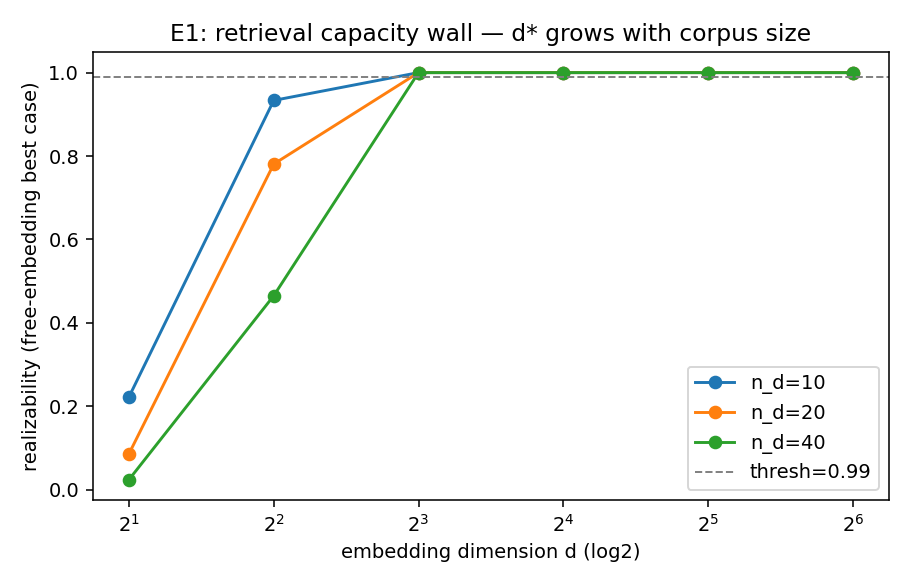
\includegraphics[width=0.32\linewidth]{figures/e1_capacity_wall.png}
\hfill
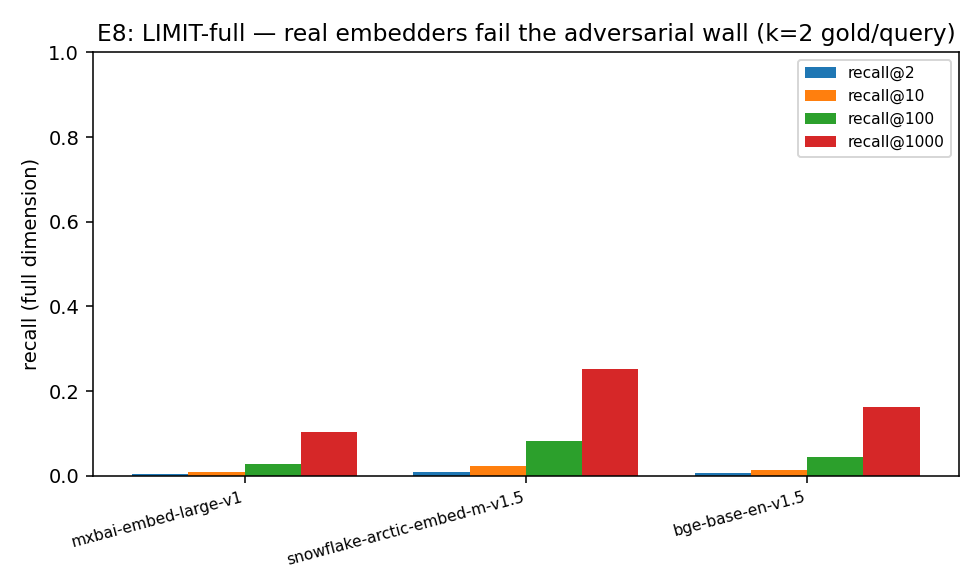
\includegraphics[width=0.32\linewidth]{figures/e8_limit.png}
\hfill
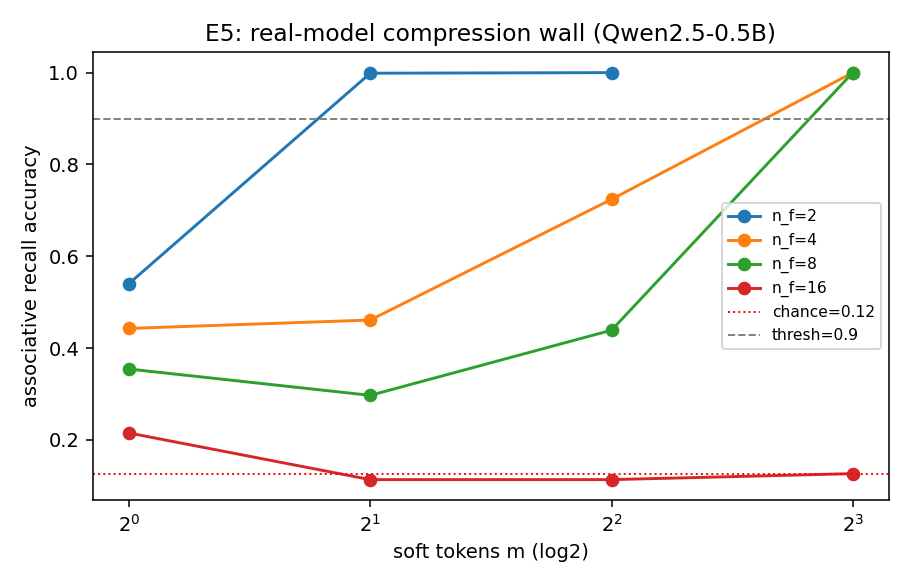
\includegraphics[width=0.32\linewidth]{figures/e5d_trained_wall.png}
\caption{\textbf{C1.} Left: the free-embedding retrieval wall---realizability jumps sharply once
$\dr$ clears a critical value that grows with corpus size $n_d$. Middle: on LIMIT, three real
embedder families all fail the adversarial pattern at full dimension. Right: a real \emph{trained}
gist/xRAG-style compressor shows the compression wall directly---critical token count $m^\star$
grows with content and $n_f{=}16$ never clears chance (red), corroborating the probe.}
\label{fig:c1}
\end{figure}

\section{Composing the two stages compounds (C2)}
\label{sec:compound}

\paragraph{Independent composition already bites.} If the two stages fail on independent items,
the pipeline recall is the product $p_R(\dr)\cdot p_C(D_c)$, so composing two sub-full stages must
underperform either one at the full budget. On a synthetic corpus that shares a budget
$B=\dr+D_c$ between the real retrieval and compression walls of Section~\ref{sec:walls}, the best
split at $B=64$ reaches only $0.559$ even though each stage alone exceeds $0.95$ at that budget---a
compounding gap of $0.389$---and the gap closes to $0.001$ by $B=192$ once both stages clear their
walls. The effect is largest exactly where deployments live, at tight budgets where neither stage
is saturated.

\paragraph{The deviation from the product law is set by a hardness correlation.} Independence is a
baseline, not a law, so we model the two per-item success events with a Gaussian copula that holds
the marginals fixed at the measured walls and varies the correlation $\rho$ between which items are
hard to retrieve and which are hard to compress. The limits are exact: $\rho\!=\!0$ recovers the
product $p_R p_C$; aligned hardness ($\rho\!>\!0$) makes failures redundant and lifts the pipeline
toward $\min(p_R,p_C)$; and misaligned hardness ($\rho\!<\!0$) is the only regime that compounds
\emph{super}-multiplicatively, pushing the pipeline below $p_R p_C$ toward the Fr\'echet floor
$\max(0,p_R+p_C-1)$. Concretely, at a balanced $32{:}32$ split the pipeline moves from $0.515$ at
$\rho=-0.5$ (below the independent $0.559$) up to $0.687$ at $\rho=+0.9$. So the sign of the
compounding is an empirical question about real corpora, which prior work left open.

\paragraph{We measure $\rho$, and it is near zero.} On a real pipeline---a truncated
\texttt{mxbai} retriever and a real-encoder compressor over one shared corpus---we record, per
query, a retrieval difficulty (gold-versus-best-distractor margin) and a compression difficulty
(the reader's correct-versus-best-other logit margin), and correlate them. Across three balanced,
sub-saturated operating points the mean $\rho_\phi$ is $+0.009$, i.e.\ essentially zero, and the
copula prediction reproduces the observed pipeline recall almost exactly: observed
$\{0.234,0.443,0.555\}$ against the product law $\{0.227,0.439,0.555\}$, a mean absolute error of
$0.0035$ (independent) or $0.0012$ (with the measured $\rho$). The reading is that real RAG, at
least on a benign corpus, lives in the multiplicative regime, so the pessimistic
super-multiplicative case needs adversarial anti-correlation that we do not see by default---which
is reassuring for allocation, since it means $p_R p_C$ is a near-exact objective to optimize.

\begin{figure}[t]
\centering
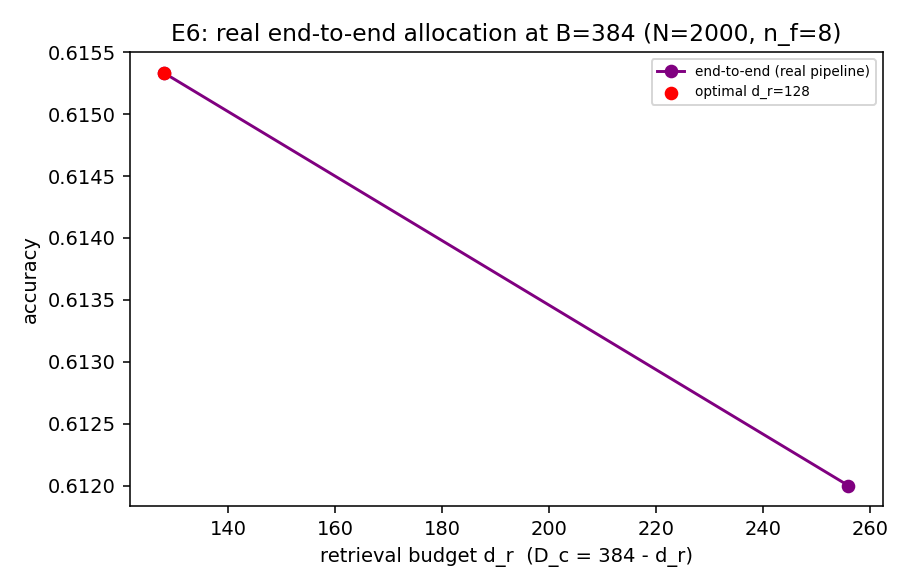
\includegraphics[width=0.48\linewidth]{figures/e6_allocation.png}
\hfill
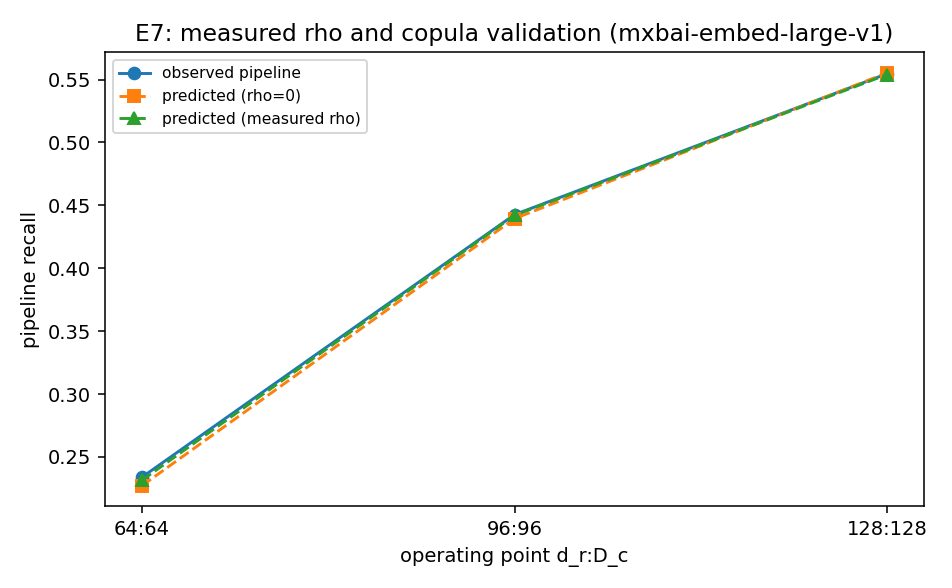
\includegraphics[width=0.48\linewidth]{figures/e7_rho.png}
\caption{\textbf{C2--C3 on real models.} Left: end-to-end accuracy versus the retrieval share of a
fixed budget---the optimum is interior, and the big-embedder/tiny-compressor corner is off it.
Right: measured $\rho\!\approx\!0$; the copula (product law) reproduces the observed pipeline recall
at every operating point.}
\label{fig:c2c3}
\end{figure}

\section{Budget-optimal allocation (C3)}
\label{sec:alloc}

\paragraph{What the budget measures.} $B=\dr+D_c$ prices one retrieval dimension against one
compression dimension. This is exact under the accounting where the stages actually compete in
deployments---per-document representation storage: the ANN index ($N\dr$ floats) and the code
cache ($ND_c$ floats) occupy the same corpus-scaled memory, so $B$ is floats per document.
Query-time compute instead prices the stages deployment-dependently (index scan $\propto N$ per
dimension; reader prefill ${\approx}2P$ FLOPs per \emph{token}, independent of slot width), so no
universal FLOP unit exists (Appendix~\ref{app:budget}). The conclusions do not hinge on the
pricing: under cost $\alpha\dr+D_c$ the optimum stays interior and the gap positive for every
$\alpha\in[\tfrac14,4]$, only its location shifting as pricing predicts (Table~\ref{tab:alpha}).

Because the pipeline is (near-)multiplicative, the optimal split of a fixed budget follows a simple
recipe: fund retrieval up to its wall $\dr^\star$, then pour the remainder into compression, since
dimensions past the retrieval wall buy almost nothing while the compressor is still starved. On the
synthetic composition this is exactly what we see---the optimal split is $48{:}(B\!-\!48)$ for all
$B\ge 96$, with a balanced $32{:}32$ preferred only when $B$ is below twice the wall---and it holds
end-to-end on real encoders. On one shared corpus with a real \texttt{mxbai} retriever and a
real-encoder compressor, the best split at $B=128$ is interior ($64{:}64$) and reaches $0.234$ while
the stages alone reach $0.63$ and $0.89$, a compounding gap of $0.392$ that shrinks to $0.137$ by
$B=256$ (Figure~\ref{fig:c2c3}, left). The practical statement is blunt: the standard configuration
of a large $\dr\!\approx\!768\!-\!1024$ embedding with a tiny $m\!\approx\!1\!-\!8$ compressor sits
far off the frontier, since it spends heavily on embedding dimensions past the retrieval wall while
the compressor overflows, and re-allocating the same budget buys accuracy for free. Concretely, on
real QA (E9, below), moving the shared budget from the deployed big-retrieval/tiny-compression
corner to the interior optimum raises answer F1 by $+0.032$ (1.5B reader) and $+0.035$ (7B) at
$B{=}256$, at identical token cost. Combined with C1,
which locates each wall cheaply by truncation, this is an actionable procedure: measure both walls,
then split the budget so retrieval is funded to $\dr^\star$ and the rest goes to compression.

\paragraph{Confirmation on a real multi-hop QA benchmark (E9).} The synthetic pipeline of E6 isolates
the mechanism, but the claim that matters is whether it survives on an actual question-answering task
with a real frozen reader. We pool every HotpotQA question's paragraphs into one shared corpus (a
genuine retrieval problem, not one isolated per question), truncate a real embedder to $\dr$ for
retrieval, select sentences into a fixed token budget by $D_c$-truncated query similarity (the
deployable, selective instantiation of compression used by RECOMP-style systems), and let a frozen
\texttt{Qwen2.5-1.5B-Instruct} answer, scored by EM/F1 over three seeds. Both claims survive on real
answer quality (Figure~\ref{fig:e9}). The allocation curve is single-peaked with an \emph{interior}
optimum: F1 rises to a peak near $\dr\!\approx\!80\!-\!96$ and then declines along a long tail out to
$\dr{=}224$, so past the optimum more retrieval budget \emph{hurts}, because it starves compression---
exactly the shape C3 predicts. And composition compounds at the tight budget: at $B=128$ the best
split reaches F1$=0.335$ against standalone references of $0.39$ (retrieval) and $0.56$ (compression),
a compounding gap of $\mathbf{0.048\pm0.007}$ F1 with all three seeds positive; the gap shrinks to
$0.009\pm0.015$ (null) by $B=256$ once both stages clear their walls, the same shrinking-with-budget
pattern as the synthetic result and consistent with the measured $\rho\!\approx\!0$. The precise
optimum location is noisy across seeds ($\dr^\star$ in $64\!-\!160$), but its interior character and
the tight-budget compounding gap are robust---the real-QA, EM/F1 counterpart of E3 and E6. The gap
is also \emph{reader-scale robust}: across a $5\times$ range of reader size (\texttt{Qwen2.5} at
1.5B, 3B, and 7B, three seeds each) the tight-budget ($B{=}128$) gap stays flat at $0.048/0.058/0.058$
F1 and the interior optimum holds at every scale---it does not vanish or reverse with reader
capability. This is the signature of an \emph{information} bottleneck rather than a reasoning one---a
more capable reader extracts more from good context, so the penalty for the evidence the two stages
discard persists (and at the looser budget grows: $0.009{\to}0.036{\to}0.027$), unlike a
context-cleanup heuristic whose benefit a stronger reader absorbs. It is also
dataset-general: on a second multi-hop benchmark (2WikiMultihopQA, three seeds) the tight-budget
gap is $0.048\pm0.014$ F1 with the same single-peaked interior optimum.

\begin{figure}[t]
\centering
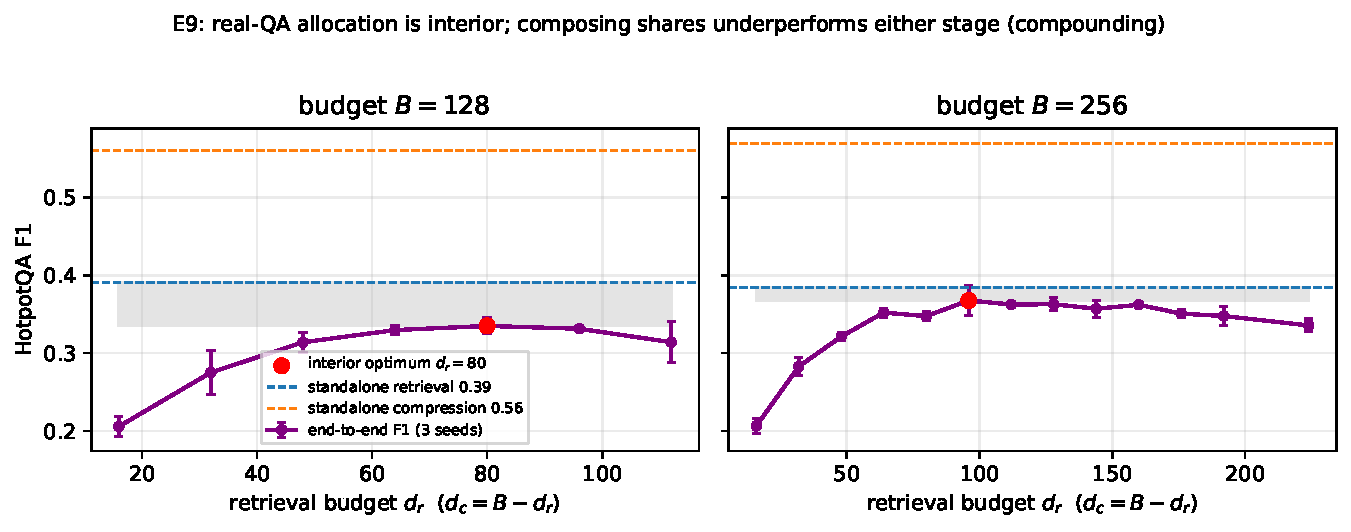
\includegraphics[width=0.92\linewidth]{figures/e9_real_qa.pdf}
\caption{\textbf{C2--C3 on real multi-hop QA} (HotpotQA, \texttt{Qwen2.5-1.5B} reader, EM/F1, three
seeds). End-to-end F1 versus the retrieval share of a fixed budget. The curve is single-peaked with
an interior optimum (red), and past it more retrieval budget hurts (it starves compression). The
shaded band is the compounding gap---the best split underperforms the weaker standalone stage---which
is positive at the tight budget $B{=}128$ ($0.048\pm0.007$ F1) and vanishes by $B{=}256$.}
\label{fig:e9}
\end{figure}

\section{When does multi-view help? The escape and its scope (C4)}
\label{sec:facet}

A natural way to beat a single-vector wall is to stop using a single vector. We test a facet-lens:
$K$ low-rank lenses, each specialized to one semantic facet (entities, numerics, relations,
negation, $\dots$), with a lightweight router sending each query to its facet's lens, so every doc
gets $K$ small codes instead of one large one at equal total budget. In the free-vector worst case
this escapes the wall cleanly. On a facet-structured pattern, routed facet-lenses realize the
relevance structure at critical budget $\dr^\star=12$ against a single vector's $24$---half the
budget---and, tellingly, a generic $K$-view MaxSim scheme with no routing is \emph{worse} than a
single vector ($\dr^\star=48$), so the lever is specialization plus routing, not multi-vector per se.
This distinguishes the facet-lens from late-interaction multi-vector retrieval
\citep{khattab2020colbert}, where the gain comes from many token vectors rather than from routing to
a facet.

We then report the honest negative: the escape does \emph{not} transfer to a strong real encoder.
Learning low-rank lenses over frozen \texttt{mxbai} embeddings of a facet-structured corpus (ten
facets), a single \emph{learned} projection ties the routed lenses---both reach mean average
precision $0.9$ at budget $40$---and the single projection actually leads at tight budgets ($0.735$
versus $0.581$ at budget $20$), while generic multiview is far behind (budget $320$). The mechanism
is instructive: a powerful pretrained encoder has already spent representational capacity making the
facets close to linearly separable, so a single learned projection can unmix them and routing adds
little, whereas the free-vector escape was a worst-case sign-rank phenomenon in which no single set
of vectors could satisfy all facet constraints at once. The consequence for practice is clean and,
we think, more useful than a method that only wins in the worst case: on real encoders the lever is
allocation (C3), not multi-view, and multi-view is not a free lunch. We therefore keep C4 as a
scoped ``when does it help'' result rather than the paper's headline, which protects the empirical
core (C1--C3) from an overclaim.

\begin{figure}[t]
\centering
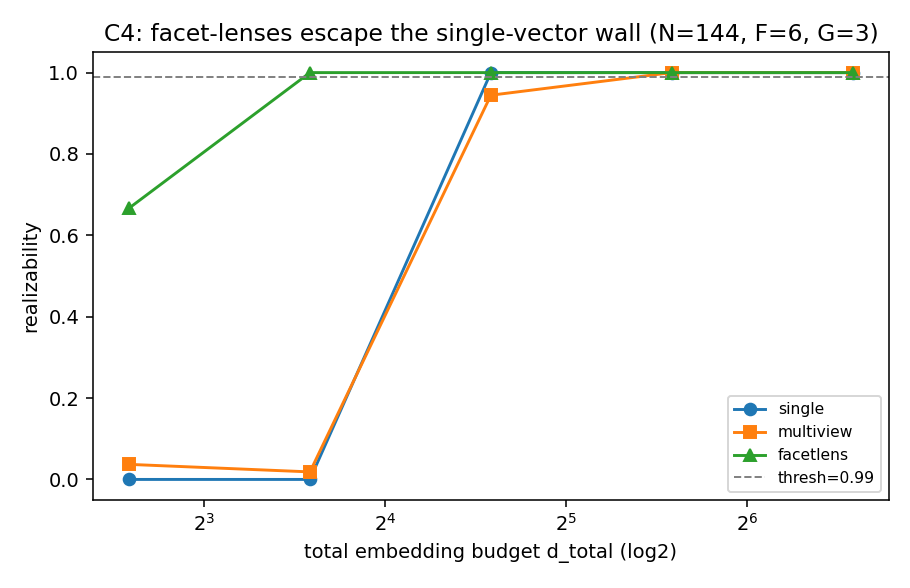
\includegraphics[width=0.45\linewidth]{figures/c4_facetlens_escape.png}
\hfill
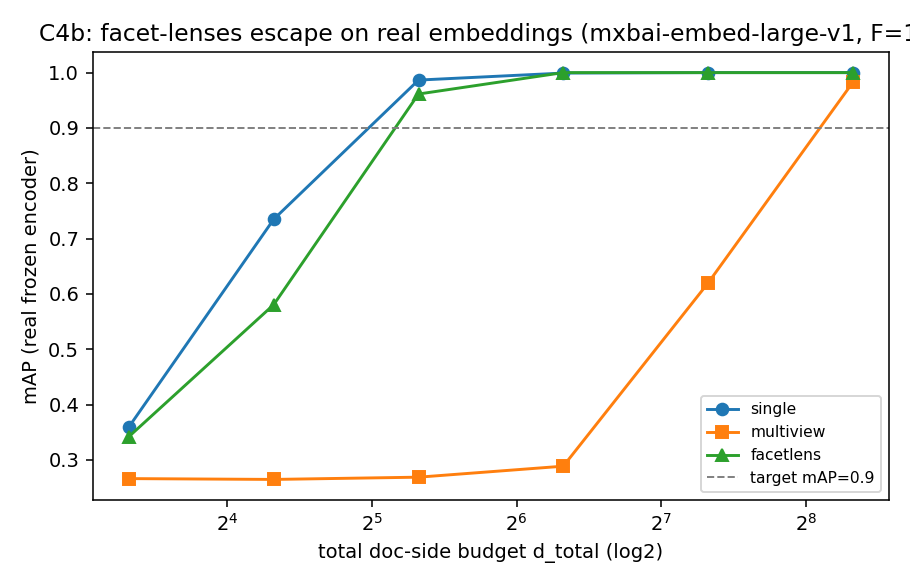
\includegraphics[width=0.45\linewidth]{figures/c4b_real_facetlens.png}
\caption{\textbf{C4 and its scope.} Left (free vectors): routed facet-lenses escape the wall at
half the budget of a single vector, while generic multiview is worse than single. Right (frozen
real encoder): the escape vanishes---a single learned projection ties the routed lenses and leads
at tight budgets---because a strong encoder has already linearized the facets.}
\label{fig:c4}
\end{figure}

\section{Discussion and limitations}

The account is deliberately a capacity characterization rather than a closed-form theorem. The
free-vector measure is a best case, so real encoders can only do worse, which is why the wall shows
up so cleanly on truncated production embeddings and on LIMIT; but it also means our
$\ceff\le\min(\cdot)$ statement is a proposition about the realizable set backed by a direct
empirical measurement of that set, not a bound with constants. Several boundaries are worth
stating plainly. The compounding experiments use controlled single-task corpora so that we can hold
the marginals fixed and vary $\rho$; the measured $\rho\!\approx\!0$ is on a benign corpus, and
whether adversarial inputs can drive the \emph{joint} $\rho$ negative---LIMIT shows retrieval can be
driven near zero, but the joint hardness correlation under such pressure is untested---is the one
genuinely open question we would flag, since a negative $\rho$ is where the pessimistic
super-multiplicative regime lives. The compression capacity is isolated with a light probe rather
than a fully-trained generative soft-token compressor, which in our hands stays at chance without a
large training budget; the probe cleanly establishes the capacity ceiling but does not model the
end-to-end training dynamics of methods like \citet{cheng2024xrag,ge2023icae}. Finally, C4's escape
is scoped out of the strong-real-encoder regime, so we do not claim multi-view as a general remedy;
we claim, more narrowly and we think more usefully, that specialization-plus-routing is what would
be needed for an escape and that a strong encoder makes it redundant.

\section{Conclusion}

We treated the retriever and the compressor of efficient RAG as two fixed-dimensional vector
bottlenecks of the same geometric form, and showed that composing them compounds: each stage has a
capacity wall that grows with content and that appears on real encoders, on a second dataset, under
optimal truncation, and on the adversarial LIMIT set; the composition underperforms either stage,
with the deviation from the product law set by a hardness correlation that we measured to be near
zero, which places real RAG in a multiplicative regime; and the resulting allocation is interior,
so the deployed habit of a large embedding with a tiny compressor is off the frontier and can be
improved at equal cost. We also tested the obvious multi-view escape and reported honestly that it
does not transfer to strong real encoders, which points the practical lever back at allocation. The
picture that emerges is a full arc---a diagnosis of the problem, an actionable allocation for it, and
a careful account of when a fancier representation would and would not help---and we hope it reframes
``efficient RAG'' as a budget-allocation problem across two coupled bottlenecks rather than two
tricks tuned in isolation.

\subsubsection*{Reproducibility statement}
Every experiment is driven by a committed YAML configuration and a fixed seed, headline claims use
at least three seeds with reported variance, and each run emits a machine-readable results file and
a human-readable summary. The capacity primitives, synthetic-corpus generators, real-encoder
truncation and probe code, the copula composition, and the facet-lens are all in the released
source, and the figures and tables here are produced directly from the committed outputs. Real-model
experiments use publicly available encoders (\texttt{mxbai-embed-large-v1},
\texttt{arctic-embed-m-v1.5}, \texttt{bge-large-en-v1.5}, \texttt{all-MiniLM-L6-v2}) and datasets
(SciFact, FiQA, LIMIT) and run on single commodity GPUs.

\bibliography{references}
\bibliographystyle{iclr2026_conference}

\appendix
\section{Summary of experiments}
\label{app:experiments}

Table~\ref{tab:exps} collects every experiment behind the claims in the main text, with the
setting and the headline number, so the results can be traced to a single row. Each corresponds to
a committed configuration and a fixed seed; headline claims use at least three seeds.

\begin{table}[h]
\caption{All experiments, their setting, and the headline result. ``Free'' denotes the
free-embedding capacity primitive of Section~\ref{sec:setup}; ``real'' denotes a frozen production
encoder. Budgets are embedding/code dimensions.}
\label{tab:exps}
\centering\small
\begin{tabular}{@{}llp{4.4cm}p{4.6cm}@{}}
\toprule
ID & Kind & Setting & Headline result\\
\midrule
E1/E1c & free & all-pairs \& random-$k$ patterns; sweep $\dr$, $n_d$; 5 seeds & sharp wall; $\dr^\star$ grows $8\!\to\!11$ as $n_d\,40\!\to\!400$; ``$d/n_d$'' law refuted ($R^2{=}0.18$)\\
E2 & free & slot-memory read; sweep $D_c$, $n_f$ & compression wall $D_c^\star\!\approx\!2n_f$\\
E4 & real & mxbai / SciFact; Matryoshka trunc.\ & recall@10 $0.09\!\to\!0.87$; flat past $\dr{=}512$\\
E4b & real & arctic-m / SciFact; Matryoshka & $97\%$ of full recall by $\dr{=}256$\\
E4c & real & mxbai / FiQA (domain shift) & $92\%$ of full recall by $\dr{=}256$\\
E4d & real & bge-large / SciFact; \textbf{PCA} trunc.\ & saturates at $\dr{=}256$ ($98.5\%$)\\
E5/E5b & real & mxbai code; light read probe & one vector $\approx$ one fact ($0.98\!\to\!0.20$); multi-token recovers to $0.99$\\
E5c & real & \textbf{bge-large} code; same sweeps & compression wall replicates ($D_c^\star$ grows with $n_f$); F6 thin-slot scope holds\\
E5d & real & \textbf{trained} gist/xRAG-style compressor (LoRA, 2000 steps) & wall confirmed directly: $m^\star{=}2{\to}8{\to}8{\to}$none for $n_f{=}2,4,8,16$; $n_f{=}16$ loss $\to\ln 8$\\
E8 & real & LIMIT; 3 embedders; 50k / 46 docs & recall@100 $=2.8/8.2/4.5\%$ (full)\\
E3 & free & shared budget $B{=}\dr{+}D_c$ & compounding gap $0.389$ at $B{=}64$\\
E3b & free & Gaussian copula over stage successes & sign of gap set by $\rho$; Fr\'echet-bounded\\
E7 & real & mxbai retriever + compressor; per-item margins & $\rho_\phi\!=\!+0.009$; product law exact to $\sim\!0.001$\\
E6 & real & mxbai; one corpus; $N{=}2000$ & gap $0.392$ at $B{=}128$; optimum interior $64{:}64$\\
E9 & real & HotpotQA; Qwen2.5-1.5B; EM/F1; 3 seeds & interior optimum; gap $0.048{\pm}0.007$ F1 at $B{=}128$, null at $256$\\
E9c/E9e & real & HotpotQA; Qwen2.5-\textbf{3B/7B}; 3 seeds & reader-robust: $B{=}128$ gap $0.058/0.058$ (flat over 1.5B/3B/7B, no reversal)\\
E9d & real & \textbf{2Wiki}; Qwen2.5-1.5B; 3 seeds & cross-dataset: gap $0.048{\pm}0.014$ at $B{=}128$; same interior optimum\\
C4 & free & facet pattern; single / multiview / routed & routed $\dr^\star{=}12$ vs single $24$; multiview $48$\\
C4b & real & frozen mxbai; 10 facets; learned lenses & single ties routed ($\dr^\star{=}40$); no transfer\\
\bottomrule
\end{tabular}
\end{table}

\section{Implementation details}
\label{app:impl}

\paragraph{Free-embedding capacity primitive.} For a target relevance pattern $A\in\{0,1\}^{M\times N}$
we optimize unconstrained document vectors $X\in\R^{N\times d}$ and query vectors $Q\in\R^{M\times d}$
with Adam on a pairwise margin loss that, per query, pushes the smallest relevant score above the
largest non-relevant score by a margin; realizability is the fraction of queries for which this
holds strictly. Because $X,Q$ are free, this upper-bounds any encoder of dimension $d$, so a wall
here is a wall for every encoder. The all-pairs pattern sets every document pair as one query's gold
set ($k{=}2$); random-$k$ draws $n_q$ distinct $k$-subsets.

\paragraph{Compression probe.} A passage of $n_f$ facts is written as $m$ codes of width $\dc$; a
query attends over the $m$ codes with a small read head and decodes the queried value with cross-entropy.
On real encoders the codes are truncated frozen embeddings, and only the light read head is trained,
which converges reliably and generalizes to held-out passages, so it measures the code's capacity
rather than the trainability of a full soft-token compressor (which, in our hands, stays at chance
without a large training budget).

\paragraph{Copula composition and measured $\rho$.} We place a Gaussian copula on the two binary
per-item success events with the marginals fixed at the measured stage recalls and correlation
$\rho$, and estimate pipeline recall by Monte-Carlo; the limits $\rho\in\{-1,0,+1\}$ recover the
Fr\'echet lower bound, the product, and the minimum. To measure $\rho$ on a real pipeline we take
the phi coefficient of the two binary successes and the Pearson correlation of two continuous
difficulty margins (retrieval gold-minus-best-distractor; compression correct-minus-best-other logit).

\paragraph{Facet-lens.} Each lens is a learned linear map $\R^{D}\!\to\!\R^{d/K}$ applied to frozen
document and query embeddings, scored by $\ip{W_q^f q}{W_d^f d}$; the router sends a query of facet
$f$ to lens $f$, so the doc-side budget $d$ is split into $K$ equal codes. Single is one full-width
lens; generic multiview keeps $K$ lenses but scores by the max over views without routing. We train
all conditions with the same objective and budget and report mean average precision.

\paragraph{Compute.} All runs use a single commodity GPU (Kaggle T4 or P100). Real-encoder runs
encode the corpus once and cache it; wall-clock ranges from seconds (LIMIT-small; the free-vector
sweeps) to about twenty-six minutes for the $50$k-document LIMIT-full sweep across three embedders.

\section{Budget accounting and exchange-rate sensitivity}
\label{app:budget}

\paragraph{Cost accounting.} Per query, a brute-force index scan costs ${\approx}2N\dr$ FLOPs
(reduced proportionally by the probed fraction under ANN); reader prefill over the compressed code
costs ${\approx}2Pm$ FLOPs for a $P$-parameter reader---per \emph{token}, with the slot width
$\dc$ free up to the reader's hidden size (the projector is negligible). Per document, storage is
$\dr+D_c$ floats regardless of deployment. A worked example shows why no universal FLOP unit
exists: at $N{=}10^6$ documents and $P{=}1.5$B, one compression token costs ${\approx}3{\times}10^9$
FLOPs at query time---roughly $1{,}500$ retrieval dimensions---whereas per-document storage prices
them $1{:}1$; at $N{=}10^9$ the same token is worth ${\approx}1.5$ dimensions. Since the rate spans
three orders of magnitude across realistic deployments, we report the storage-exact budget and
verify below that the paper's conclusions are insensitive to the rate.

\paragraph{Exchange-rate sensitivity.} Using E6's measured per-stage curves and composing by the
product law that E7 validates to ${\sim}10^{-3}$, we re-derive the optimum under cost
$\alpha\dr+D_c$ for $\alpha\in\{\tfrac14,\tfrac12,1,2,4\}$ at a tight and a loose budget
(Table~\ref{tab:alpha}). At every $\alpha$ the optimum allocates substantial budget to both stages
and strictly dominates both all-in allocations by a wide margin, and the compounding gap stays
positive; only the optimum's location moves, in the direction pricing predicts (dearer retrieval
dimensions shift it toward compression).

\begin{table}[h]
\caption{Exchange-rate sensitivity of the allocation conclusions (E6 curves, product composition).
``All-in'' = the full budget to one stage (other at the grid minimum); gap = compounding gap vs
the standalone references. The optimum is interior and the gap positive for every $\alpha$.}
\label{tab:alpha}
\centering\small
\begin{tabular}{@{}ccccccc@{}}
\toprule
$\alpha$ & budget & optimum $(\dr,D_c)$ & pipeline & all-in-R & all-in-C & gap\\
\midrule
$0.25$ & tight / loose & $(64,64)$ / $(128,128)$ & $0.227$ / $0.557$ & $0.130$ / $0.134$ & $0.073$ / $0.105$ & $+0.214$ / $+0.079$\\
$0.5$  & tight / loose & $(64,64)$ / $(128,128)$ & $0.227$ / $0.557$ & $0.118$ / $0.130$ & $0.073$ / $0.105$ & $+0.214$ / $+0.079$\\
$1$    & tight / loose & $(64,64)$ / $(128,128)$ & $0.227$ / $0.557$ & $0.069$ / $0.118$ & $0.073$ / $0.105$ & $+0.397$ / $+0.133$\\
$2$    & tight / loose & $(32,128)$ / $(128,128)$ & $0.244$ / $0.557$ & $0.069$ / $0.118$ & $0.105$ / $0.116$ & $+0.123$ / $+0.067$\\
$4$    & tight / loose & $(32,128)$ / $(128,128)$ & $0.244$ / $0.557$ & $0.069$ / $0.118$ & $0.116$ / $0.118$ & $+0.123$ / $+0.067$\\
\bottomrule
\end{tabular}
\end{table}

\end{document}
